\section{End of Chains}

Thus far we only saw the beginning and the middle of the chains.
It is not clear how the chains will develop for larger values of $\beta$.
This section will investigate how the chains develop in those areas.

\begin{figure}
	\centering
	\subfloat[Larger values for $\beta$]{
		\includegraphics[width=.45 \textwidth]{61_MinimalRepr_Halved/2D_Period_Chain_Ends/result.png}
		\label{fig:arch.chainend.1}
	}
	\subfloat[Even larger values for $\beta$]{
		\includegraphics[width=.45 \textwidth]{61_MinimalRepr_Halved/2D_Period_Chain_Ends_Cont/result.png}
		\label{fig:arch.chainend.2}
	}
	\caption[2D scans of periods in the archetypal model showing the end of the chains]{
		2D scans of periods in the adjusted archetypal model showing the end of the chains of the same period.
		(a) shows the 2D scan for larger values of $\beta$ where ``type B'' regions start missing from the chain of period $16$.
		(b) shows the 2D scan for even larger values of $\beta$ where the chain is no longer connected.
	}
\end{figure}

\Cref{fig:arch.chainend.1} shows a 2D scan of the periods of the adjusted archetypal model where the ``type B'' parameter regions in the chains are visible.
We can see that the ``type B'' parameter region between the ``type A'' parameter region marked with point $I_{16}$ and the ``type A'' parameter region marked with point $K_{16}$ is missing.
There should have been the parameter region $\P_{\A^3\B^5\C^2\D^6, \A^2\B^6\C^3\B^5}$ according to the rules laid out in \Cref{sec:arch.dynamics}.

Furthermore, the chain is completely disconnected when looking at even higher values of $\beta$.
\Cref{fig:arch.chainend.2} shows this.
The parameter region $\P_{\A\B^7\C\D^7}$ marked with $M_{16}$ is the predicted last ``type A'' parameter region of the chain with period $16$.
It is not connected to the second last parameter region $\P_{\A^2\B^6\C^2\D^6}$ marked with $K_{16}$.

This violates the rules and our expectation for the archetypal model.
But \Citeauthor{akyuz2022} observed the same behavior in the original model in his thesis.
He also looked at a chain of parameter regions with period $16$.
The chain behaved according to the rules up to the second last ``type A'' parameter region, $\P_{\A^2\B^6\C^2\D^6}$.
His hypothesis is that the scan of the periods done here is a two-dimensional one, while the model has more dimensions.
So choosing a different parameter plane for the 2D scan of the periods might reveal a perfect chain with period $16$~\cite{akyuz2022}.
This could also be the case here, since the archetypal model has $5$ parameters and the period scan is done in two dimensions also.
We will expand on this in \Cref{chap:outlook}.
